\documentclass[11pt, a4paper, oneside, portrait]{report}
\usepackage[utf8]{inputenc}
\usepackage[T2A, T1]{fontenc}
\usepackage[british, french, russian]{babel}
\usepackage[style=ieee]{biblatex}
\usepackage[most]{tcolorbox}
\usepackage{graphicx}
% \usepackage{animate}
\usepackage{xurl}
\usepackage{setspace}
\usepackage{ragged2e}
\usepackage{indentfirst}
\usepackage{mathptmx}
\usepackage{pdfpages}
\usepackage{geometry}
\usepackage{amsmath}
\usepackage{amssymb}
\usepackage{txfonts}
\usepackage{multicol}
\usepackage{fancyhdr}
\usepackage{wrapfig}
\usepackage{array}
\usepackage{float}
\usepackage{alltt}
\usepackage{tabularx}
\usepackage{caption}
\usepackage{fancyvrb}
\usepackage{fvextra}
\usepackage{enumitem}
\usepackage{bigfoot}
\usepackage{hyperref}
\geometry{
    a4paper,
    top=2cm,
    bottom=2cm,
    right=2cm,
    left=2cm
}
\hypersetup{
    colorlinks = true,
    linkcolor = blue,
    urlcolor = blue,
    filecolor = blue,
    citecolor = blue
}
\pagestyle{fancy}
\fancyhf[HC]{\textbf{MU4MEN01 --~Projet d'Optimisation}}\fancyhf[HL]{\thepage}\fancyhf[HR]{\thepage}
\fancyhf[FC]{\thepage}
% \addbibresource{References.bib}
\title{\textbf{MU4MEN01 --~Projet d'Optimisation}}
\author{AKIL Adam, BUCLET Zeca, NOCHÉ Kévin} % Mettre ton nom de famille, Zeca.
\date{\today}


\begin{document}
    \selectlanguage{french}
    \maketitle\thispagestyle{empty} % Flemme de faire plus sophistiqué.
    \newpage\tableofcontents\thispagestyle{empty}

    \newpage\setcounter{page}{1} % Démarrer le rapport à partir de cette page.


    \section*{Introduction}\addcontentsline{toc}{section}{Introduction}
        Dans ce présent document, nous allons étudier un modèle représentant un train, sa consommation, sa batterie et comment optimiser deux choses:

        ---~La capacité de ladite batterie.

        ---~La chute de tension maximale aux bornes du train, sachant que nous ne devons pas atteindre moins de $500$~V aux bornes du train.

        Le modèle auquel nous nous intéressons a été codé en python (le code est joint au document), et prend en compte, de façon non-exhaustive, les déplacements du train, sa vitesse, son accélération, sa puissance consommée et la puissance de la LAC (ligne aérienne de contact).
        Le fichier \texttt{marche.txt}, qui nous a été remis dès le début du projet, indique les déplacements du train en fonction du temps.
        De rapides et simples calculs nous permettent de trouver la vitesse du train, puis son accélération, primordiales pour la suite du projet.

    \section*{La fonction \texttt{Simulation()}}\addcontentsline{toc}{section}{La fonction \texttt{Simulation()}}
        \subsection*{Sans Batterie}\addcontentsline{toc}{subsection}{Sans Batterie}
        \subsection*{Avec Batterie}\addcontentsline{toc}{subsection}{Avec Batterie}


    \section*{Monte-Carlo}\addcontentsline{toc}{section}{Monte-Carlo}


    \section*{Algorithme NSGA-II}\addcontentsline{toc}{section}{Algorithme NSGA-II}
        L'algorithme génétique NSGA-II (\emph{Non-Dominated Sorting Generic Algorithm 2}) permet de trouver les meilleures solutions dans un contexte donné de façon assez efficace.
        Cet algorithme génère une population de taille $N$ d'individus (les solutions), puis recherche au sein de cette population les \guillemotleft{}~solutions non-dominées~\guillemotright{}, et les range en suivant cette ordre:

        ---~En premier, les solutions non-dominées, c'est-à-dire celles qui dominent toutes le autres, les meilleures de la population.

        ---~En deuxième, les solutions non-dominées qui restent, en ayant retirées les solutions précédentes de la population de départ.

        ---~ En troisième, les solutions non-dominées restantes, en ayant retirées toutes les précédentes de la population de départ.

        ---~On continue jusqu'à épuisement des individus dans la population de départ.

        Ayant maintenant à notre diposition un classement des individus selon leurs performances, on sélectionne les $50\%{}$ meilleurs dans ce classement, puis les croisons afin de créer la génération suivante.
        Puis le cycle recommence, pour un total de $N$ itérations.

        Il faut savoir que NSGA-II, demandant un classement des solutions selon leur dominance, doit utiliser une fonction qui classe les solutions selon cette ordre. Pour ceux qui regarderait notre code, il s'agit de la fonction \texttt{non\_dominant\_sort()} (voir figure \ref{fig:non_dominant_sort}).

        \begin{figure}[H]
            \centering
            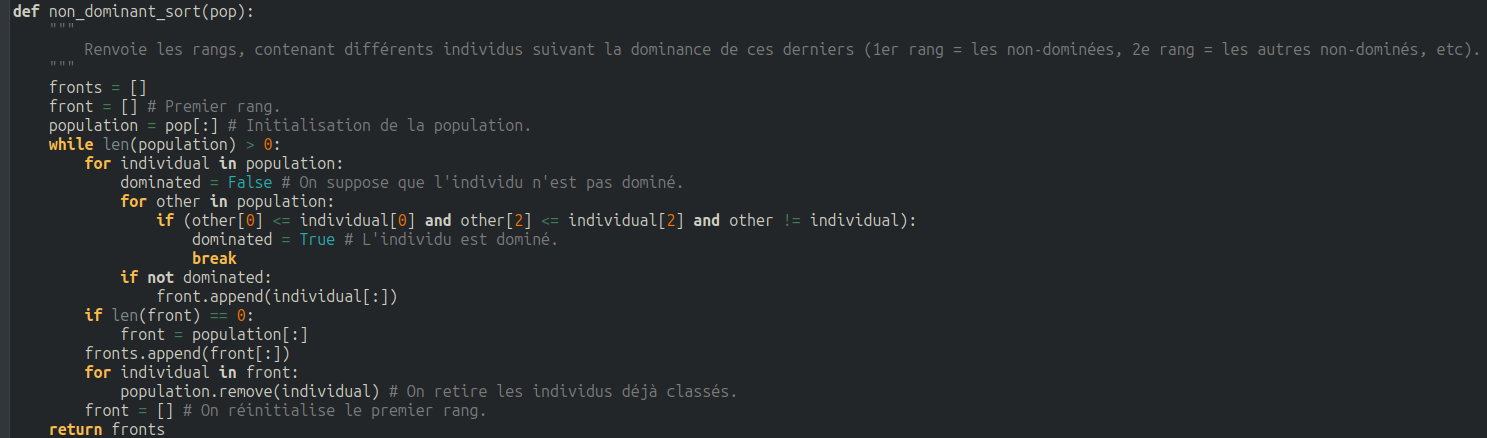
\includegraphics[width=\textwidth]{Figures/non_dominant_sort.png}
            \caption{Code de la fonction du classement en fronts.}
            \label{fig:non_dominant_sort}
        \end{figure}

        Et, pour sélectionner les $50\%{}$ meilleurs, nous utilisons la fonction ci-dessous:

        \begin{figure}[H]
            \centering
            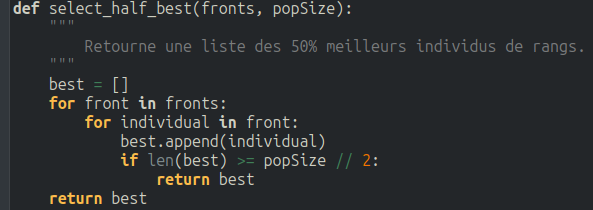
\includegraphics[width=0.75\textwidth]{Figures/select_half_best.png}
            \caption{Sélection des $50\%{}$ meilleurs.}
            \label{fig:non_dominant_sort}
        \end{figure}

        Comme affiché sur la figure \ref{fig:NSGA2}, les solutions intéressantes pour notre batterie semblent se trouver aux alentours de $1$ ou $2$~kWh, pour un seuil vers les $300$~kW et une chute de $200$~V (les points rouges représentant la dernière génération créée par notre algorithme).
        Suivant la simulation, les résultats peuvent énormément changer, et il est conseiller de relancer plusieurs fois l'algorithme afin de trouver des solutions potentiellement meilleures.
        Par ailleurs, étant donné l'absence de \guillemotleft{}~\emph{crowding\_distance}~\guillemotright{}, nommé \guillemotleft{}~critère de distance~\guillemotright{} en français, nos solutions tendent à se rassembler en un amas compact; augmenter la mutation peut sensiblement améliorer ce problème.

        \begin{figure}[H]
            \centering
            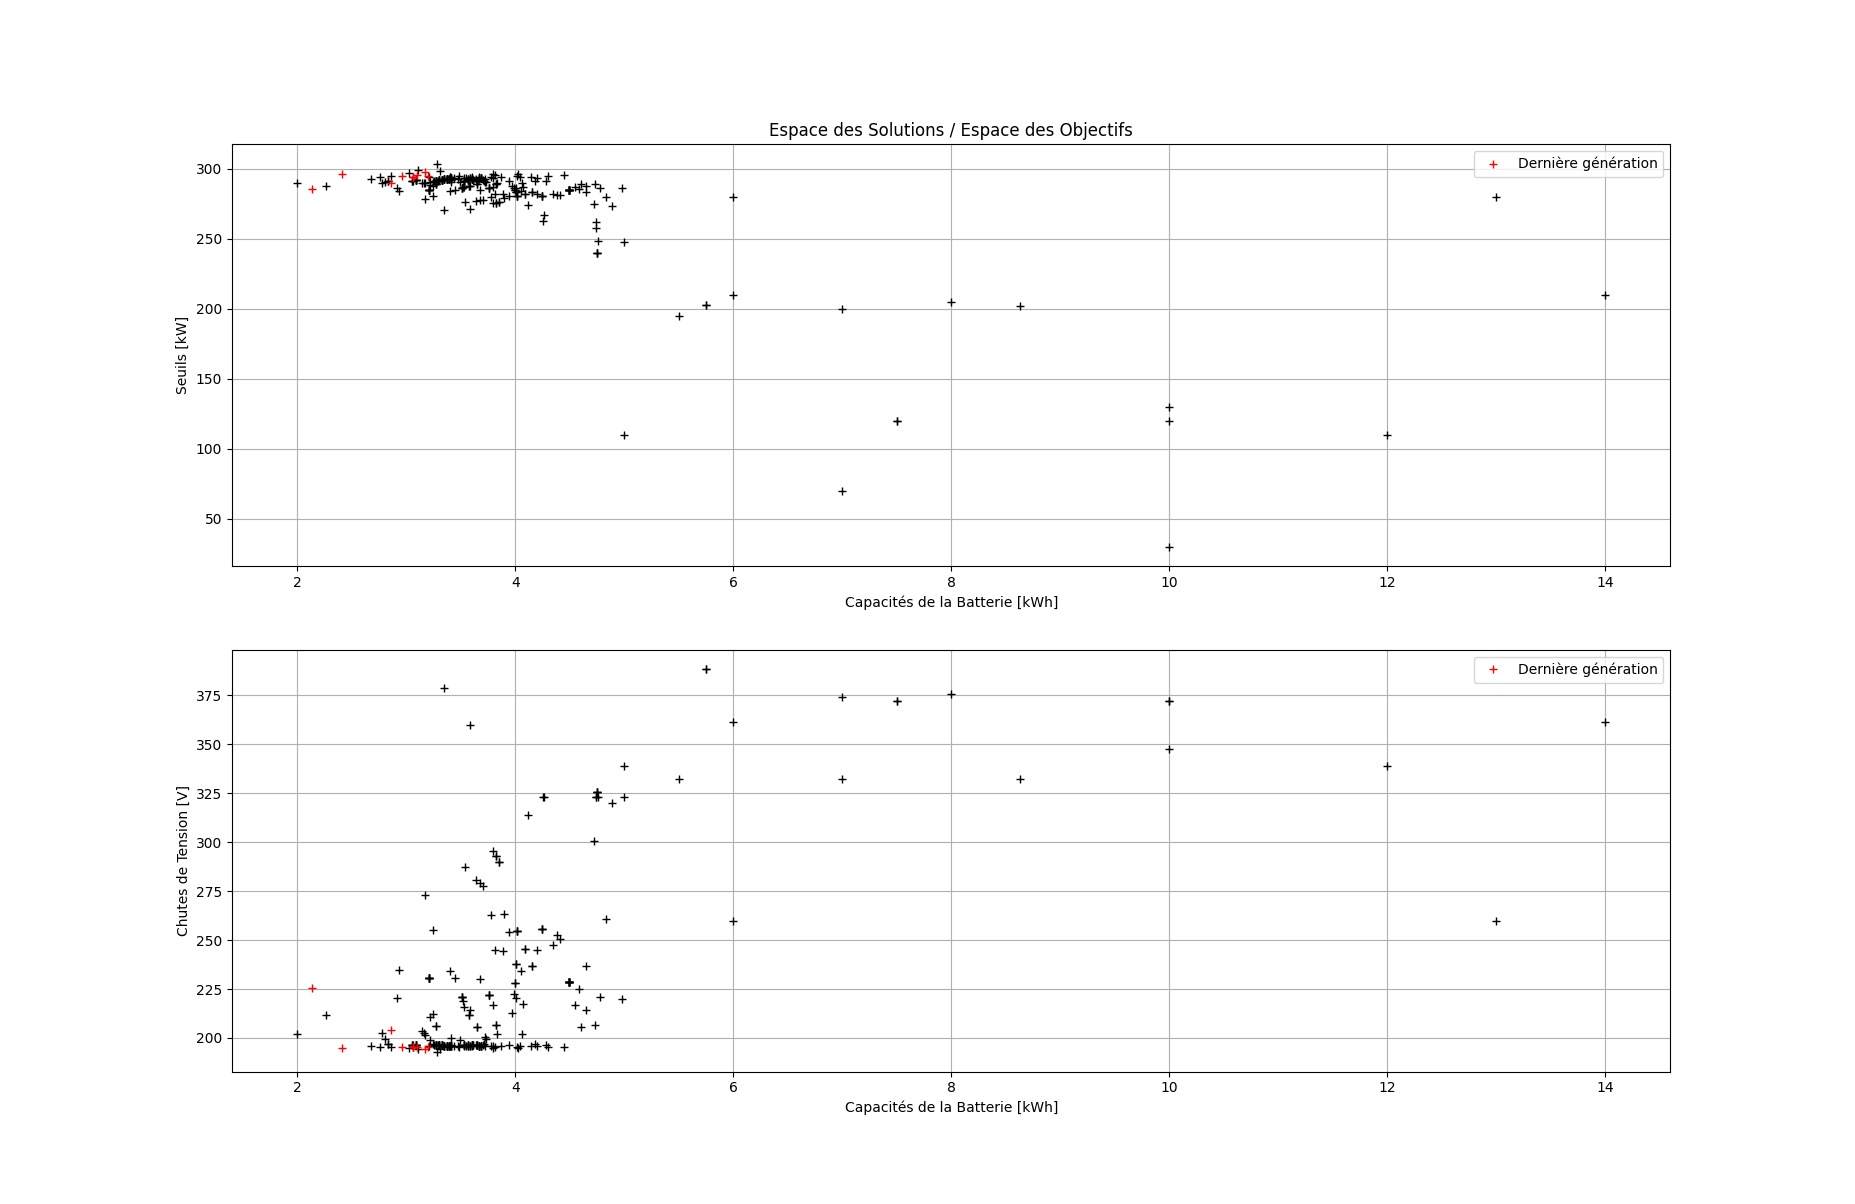
\includegraphics[width=0.75\textwidth]{Figures/NSGA-II.png}
            \caption{Résultats de l'algorithme NSGA-II.}
            \label{fig:NSGA2}
        \end{figure}


    \section*{Conclusion}\addcontentsline{toc}{section}{Conclusion}


\end{document}

% Simulation(10000, 400000, True)
